\documentclass[11pt,a4paper]{article}
\usepackage[utf8]{inputenc}
\usepackage[T1]{fontenc}
\usepackage{amsmath,amsfonts,amssymb}
\usepackage{apacite}
\usepackage{natbib}
\usepackage{graphicx}
\usepackage{booktabs}
\usepackage{threeparttable}
\usepackage{array}
\usepackage{url}
\usepackage{hyperref}
\usepackage[margin=2.5cm]{geometry}
\usepackage{setspace}
\usepackage{comment}
\usepackage{outlines}
\onehalfspacing

\newcommand{\Var}{\text{Var}}
\newcommand{\Cov}{\text{Cov}}

% Define \sym command for significance stars from esttab
\newcommand{\sym}[1]{{#1}}

\title{How Much Do CEOs Matter? Correcting for Small-Sample Bias in Fixed-Effect Estimates\thanks{Project no. 144193 has been implemented with the support provided by the Ministry of Culture and Innovation of Hungary from the National Research, Development and Innovation Fund, financed under the KKP\_22 funding scheme. This project was funded by the European Research Council (ERC Advanced Grant agreement number 101097789). Telegdy received support from the Hungarian Scientific Research Fund – OTKA, contract number 143346. The views expressed in this research are those of the authors and do not necessarily reflect the official view of the European Union or the European Research Council.}}

\author{Miklós Koren\thanks{Central European University, ELTE Centre for Economic and Regional Studies, CEPR and CESifo. E-mail: korenm@ceu.edu} \\
        Krisztina Orbán\thanks{Monash University.} \\
        Álmos Telegdy\thanks{Corvinus University of Budapest. E-mail: almos.telegdy@uni-corvinus.hu}}

\date{October 2025}

\begin{document}

\maketitle
\thispagestyle{empty}

\begin{abstract}
How much do individual CEOs contribute to firm performance? Studies typically estimate CEO fixed effects and analyze their second moments to quantify the importance of CEO heterogeneity. We show that small-sample noise systematically biases these second moments even when mean effects are unbiased, leading researchers to overstate CEO contributions and observe spurious pre-trends in event studies. We develop a placebo-controlled method that identifies and removes these biases without modeling the full error process. The method constructs matched control transitions in firms that do not change CEOs, replicating the spell-length design of actual transitions. Placebo moments recover the bias terms, which are then subtracted from treated estimates to yield debiased variances, covariances, and regression slopes. Monte Carlo experiments confirm the method removes bias across scenarios with persistent shocks, short tenures, and unbalanced panels. Applying the method to 60,000 CEO transitions in Hungarian private firms (1992--2022), we find naive estimates overstate CEO contributions to revenue variance by more than half (60 percent naive versus 29 percent corrected) and generate entirely spurious pre-trends. Debiased estimates reveal immediate and persistent CEO effects with no anticipatory patterns, suggesting that much of the apparent gradual adjustment in naive estimates is a mechanical artifact of small-sample bias. The method is broadly applicable to any setting where analysts use estimated fixed effects with short spells.
\end{abstract}

\textbf{Keywords:} CEO value, CEO-Firm Fixed Effects, Bias Correction

\textbf{JEL Classification:} C23, D24, G34

\clearpage
\setcounter{page}{1}

%%%%%%%%%%%%%%%%%%%%%%
\section{Introduction}
%%%%%%%%%%%%%%%%%%%%%%

The impact of individual CEOs on business practices and firm performance is a widely studied question in economics, corporate finance, and management. In absence of direct measures of CEO characteristics relevant for firm outcomes, studies often include CEO fixed effects to capture variations in latent CEO skills \citep{Bertrand2003-io, crossland2011differences, quigley2015has}. Under the standard assumption of ``random mobility,'' that is, CEO moves are unrelated to past and future performance shocks of the firm, the mean of estimated CEO fixed effects is unbiased. 

Most applied work, however, is concerned with the second moments of the estimated fixed effects. First, variance decompositions reveal how much CEO effects contribute to the variance of certain firm outcomes, such as revenue or profitability. Second, to understand the mechanisms through which CEOs affect firm outcomes, the estimated CEO effect is often used to assess its effect on other variables, which is based on the covariance. For example, whether firms led by better CEOs are more profitable \citep{mackey2008effect} or how much risk they take \citep{schoar2024effect}. Third, dynamic covariances are used in event studies to assess how outcomes evolve before and after CEO transitions, as a way to test for pre-trends and to understand post-transition dynamics \citep{schoar2024effect}. 

All these second moments are biased by small-sample noise in the estimated CEO effects, even under credible identification assumptions \citep{andrews2008high,gaure2014correlation,Bonhomme2023-dx}. This is not a nuisance, but has important implications for the interpretation of empirical results. Perhaps most intuitively, small-sample bias overstates the role of CEOs in explaining firm performance. Second, it distorts the covariance of CEO quality with firm outcomes, biasing estimates of how CEOs affect operational decisions. And, as we show below, the bias introduces spurious pre-trends and distorts post-transition dynamics in event studies.

Correcting for small-sample bias is challenging. Existing methods are either ad hoc, such as leave-one-out adjustments \citep{kline2020leave}, or highly structural: estimate the bias from the variance-covariance of shocks and the design matrix and then apply Empirical Bayes shrinkage \citep{andrews2008high,Bonhomme2023-dx,kline2024firm}. While powerful, these require estimating many components and re-deriving formulas for each target second moment.

Our approach is different: we create a placebo-controlled experiment. For each firm that truly changes CEOs, we find a group of comparable non-changing firms, and use this placebo control group to estimate the mechanical noise in the second moments.\footnote{This step in the spirit of \cite{jarosiewicz2023revisiting}, who compare the replicated results of  \cite{Bertrand2003-io} with placebo regressions.} Under weak assumptions, the placebo group can be used to measure the exact bias in variance, covariance, and dynamic covariance. The difference in second moments between the treated and the placebo groups yields debiased estimates, without having to model and estimate the full variance-covariance structure of errors.

We illustrate our method in Monte Carlo experiments that vary the severity of the bias problem across six scenarios: a baseline with balanced panels and independent shocks, extensions to long panels, persistent shocks, unbalanced spell lengths, excess variance in treated firms, and a scenario combining all complications. In the baseline, naive and debiased estimates coincide, confirming the method imposes no distortion when bias is minimal. With persistent shocks, the naive standard deviation of CEO effect changes is upward biased by 23 percent, and spurious pre-trends emerge even though the true pre-trend is zero by construction. The placebo correction removes these artifacts across all scenarios, recovering the true parameters even when short tenures, persistent shocks, and excess variance are all present simultaneously.

We apply the method to the universe of Hungarian private firms from 1992 to 2022, examining revenue dynamics around 60,000 CEO transitions. Naive estimates suggest that CEO effects explain 60 percent of revenue variance. The placebo-corrected estimate shows this is severely upward biased: the true contribution is 29 percent—substantial, but less than half the naive estimate. The debiased event studies reveal no pre-trends in revenue, confirming that the strong pre-trends in naive estimates are entirely spurious. CEO effects on revenue are immediate and persistent: the impact appears in the year of transition and remains stable thereafter, with no evidence of gradual adjustment. We also find that export behavior is contemporaneously correlated with CEO quality, with better CEOs generating an immediate 4 percentage point increase in the probability of exporting.

%% now we explain everything in a bit more details

The main idea of our correction method is the creation of pseudo CEO transitions in the data\footnote{This step in the spirit of \cite{jarosiewicz2023revisiting}, who compare the replicated results of  \cite{Bertrand2003-io} with placebo regressions.} We take firms with CEO transitions, record their event window. The event window is the period encompassing the years under the CEO prior to the CEO change and the period under the new CEO post the change. We match these firms to firms born in the same year, belonging to the same sector, that however do not experience a CEO transition during the years of the event window. Then, we assign to the control firms a placebo CEO transition happening in the same year as the treated firm experiences the true CEO transition.\footnote{In addition to addressing the limited mobility bias, our approach has the advantage of creating a control group that is more similar to the treated firms than the universe of firms}. We compute second moments of the CEO fixed effect on the matched sample. The estimated `effects' for these pseudo-CEOs reveal the noise in the fixed effects estimation. By comparing actual CEO transitions to these placebo transitions, we can correct the fixed effects estimates for noise, isolating the true CEO contribution.

Our method relies on two key assumptions about the nature of shocks. First, we assume strict exogeneity, that is, that error terms are mean independent of the CEO path for all time periods. This ensures that the estimated CEO effects are mean unbiased. Second, we assume that the autocovariance of errors is the same between treated and control firms, up to a scalar multiplier. In other words, we allow for treated firms to be more volatile than control firms, but we assume that the temporal correlation structure of shocks is the same. We call this assumption ``proportional autocovariance.'' This assumption is similar in spirit to the parallel trends assumption in difference-in-differences designs. Other than these two assumptions, we make no further restrictions on the error process, the number and length of CEO spells, or the heterogeneity of CEO effects. 

To understand how these assumptions help debias the variance-covariance of estimated CEO effects, note that the bias terms are weighted sums of the autocovariances of errors, with weights depending on the research design, including the spell length of CEOs at each firm. The placebo design ensures that treated firms and control firms have the same spell-length distributions, and therefore the same weights. The proportional autocovariance assumption then implies that the bias terms are the same up to a scalar. And because covariance is a bilinear operator and variance is additive under strict exogeneity, the bias terms can be ``precomputed'' in the placebo group and simply subtracted from the treated moments.\footnote{This is not true for nonlinear transformations of variances and covariances, such as correlations and regression slopes. In these cases, we first debias all underlying variances and covariances and only then form the ratio.} In summary, the placebo group, by construction, has no CEO effects, so the variance and covariance of estimated placebo effects identify the bias terms. Subtracting these from the treated moments yields debiased estimates.

%literature
Our work connects to the broader literature on management practices and firm performance. Randomized controlled trials demonstrate that management training and consulting improve firm performance \citep{bloom2013does, mckenzie2021small}, but these interventions change practices rather than people. Whether replacing managers generates similar gains remains contentious. Evidence from public sector organizations suggests modest manager effects \citep{fenizia2022managers, janke2024role}, while studies of family firms find larger impacts when professional managers replace family members \citep{bennedsen2007inside, sraer2007performance}. Our results for private firms fall between these extremes: CEOs matter, but less than raw correlations suggest.

Methodologically, our paper builds on the two-way fixed effects literature in labor economics that decomposes wages into worker and firm components \citep{Abowd1999Econometrica, Card2018JoLE}. These studies face similar challenges from limited mobility creating small-sample bias \citep{andrews2008high} and have developed bias-correction methods \citep{Bonhomme2023-dx, gaure2014correlation}. We adapt this framework to the CEO-firm setting but add placebo controls to separate signal from noise. This approach is valuable when studying managers who, unlike workers, have few observations per individual, making traditional bias-correction methods less effective. Recent work has documented apparently increasing CEO effects over time \citep{quigley2015has}, but these studies do not account for the mechanical noise we identify. \citet{lippi2014corporate} find that concentrated ownership in Italian firms distorts executive selection and reduces productivity by 10\%, providing motivation for our framework separating owner and CEO decisions.

%%%%%%%%%%%%%%%%%%%%
\section{The Econometric Problem}
%%%%%%%%%%%%%%%%%%%%

Let firm $i$ in year $t$ have outcome
\begin{equation}\label{eq:model1}
  y_{it} = z_{m(i,t)} + e_{it},\qquad \mathbb E[e_{it}|z_{is}]=0,
\end{equation}
where $z_{m(i,t)}$ collects the CEO effect at time $t$ and $e_{it}$ is a shock. We assume that $z_{m(i,t)}$ is piecewise constant, changing only when the CEO changes and that $e_{it}$ is mean independent of the CEO path for all $s$ (``strict exogeneity'' or ``random mobility'').

Under the strict exogeneity assumption, the ordinary least squares (OLS) estimator of $z_m$ is unbiased. Equation \eqref{eq:model1} can be rewritten as a dummy-variable regression 
$$
y_{it} = \sum_{n} z_n D_{m(i,t)=n}  + e_{it},
$$
and the first-order condition for the OLS estimator $\hat z_n$ is
$$
0 = \sum_{i,t:m(i,t)=n} (y_{it} - \hat z_n),
$$
or 
$$
\hat z_n = \frac{1}{T_n} \sum_{i,t:m(i,t)=n} y_{it} = z_n + \frac{1}{T_n} \sum_{i,t:m(i,t)=n} e_{it},
$$
where $T_n$ is the number of observations with CEO $n$. The estimator is unbiased because $\mathbb E[\hat z_n|z_n] = z_n$. The estimator, however, is only consistent as $T_n\to\infty$, that is, as the number of observations per CEO grows large. In practice, many CEOs have short tenures, so $\hat z_n$ contains substantial noise.\footnote{The mean CEO tenure (standard deviation) is 13.8 (1.7) years in US small and medium-sized companies \citep{simsek2007ceo}, 8.1 (5.8) years in US public companies \citep{brookman2009ceo}. The large standard deviations demonstrate that many CEOs have only a few years of tenure.} 

Econometric applications often require the second moments of $\hat z_n$, for example, to estimate the variance of CEO effects or to run regressions of an outcome $y_{it}$ on $\hat z_n$. The former could inform us about the importance of CEO heterogeneity (REFs), while the latter could inform us about the effect of CEO quality on firm performance and firm policies (REFs). 

The small-sample error contaminates all second moments of $\hat z_n$. A well-known example is ``limited mobility bias'' \citep{andrews2008high}, which states that in a two-way fixed effects model of worker and firm effects, the variance of both effects is biased upwards and their correlation is biased downwards.


\newenvironment{example}{\par\noindent\textbf{Example.}\ }{\par}

\paragraph{Estimation and the bias problem.} In practice, we estimate CEO effects $z_m$ as the average outcome during each manager's tenure (the least-squares dummy variable or LSDV estimator). When manager $m$ is observed for $T_m$ periods, the estimate is
$$
\hat z_m = \frac{1}{T_m}\sum_{i,t:m(i,t)=m} y_{it} = z_m + \frac{1}{T_m}\sum_{i,t:m(i,t)=m} e_{it}.
$$
Under strict exogeneity, $\hat z_m$ is unbiased: $\mathbb E[\hat z_m] = z_m$. However, the estimator is only consistent as $T_m\to\infty$. With short tenures, $\hat z_m$ contains substantial noise from the averaged shocks.

This small-sample noise contaminates all second moments of $\hat z_m$. Consider three common applied use cases:

\textit{Variance decompositions.} Researchers estimate $\Var(\hat z_m)$ to quantify the importance of CEO heterogeneity. But $\Var(\hat z_m) = \Var(z_m) + \Var(\text{noise})$, systematically overstating the role of CEOs.

\textit{Covariances with other variables.} Researchers regress firm outcomes or policies on $\hat z_m$ to understand mechanisms. But $\Cov(\hat z_m, y_{it})$ includes spurious correlation between the noise component of $\hat z_m$ and $y_{it}$.

\textit{Event studies.} Researchers examine outcome dynamics around CEO transitions by contrasting post-transition and pre-transition averages. These contrasts embed noise that can generate spurious pre-trends and distorted post-transition dynamics, even when the true causal effect has no pre-trend.

The key insight is that the bias depends on the \emph{design}: the spell lengths (how long each CEO is observed) and the autocorrelation structure of shocks. When spells are short and shocks are persistent, noise inflates variances, distorts covariances, and creates spurious dynamics.

\paragraph{Bias terms.} We formalize the bias for a typical event-study contrast. Consider firms with a CEO transition, where we observe $T_1$ periods before the transition (under the old CEO) and $T_2$ periods after (under the new CEO). The contrast of interest compares an outcome from the post period to an outcome from the pre period, for example, the change from the year before transition ($t=-1$) to three years after ($t=+3$). 

For a general linear contrast, let $\Delta \hat z_i$ denote the estimated change in CEO effects for transition $i$, and $\Delta y_i$ the corresponding change in outcomes. In applications with heterogeneous spell lengths and event windows, firms are grouped into design groups $g=1,\ldots,G$, each with $N_g$ transitions. The sample covariance and variance are
\begin{align}
\widehat{\Cov}(\Delta y_i,\Delta \hat z_i) &= \sum_{g=1}^G \frac{N_g}{N} \widehat{\Cov}_g(\Delta y_i,\Delta \hat z_i),\\
\widehat{\Var}(\Delta \hat z_i) &= \sum_{g=1}^G \frac{N_g}{N} \widehat{\Var}_g(\Delta \hat z_i).
\end{align}

Under the model assumptions, these moments have expectation
\begin{align}
\mathbb E\widehat{\Cov}(\Delta y_i,\Delta \hat z_i) &= \Bar\lambda + A,\\
\mathbb E\widehat{\Var}(\Delta \hat z_i) &= \Bar\lambda + B,
\end{align}
where $\Bar\lambda$ is the average variance of true CEO effect changes across groups (the object of interest), and $A$ and $B$ are \emph{bias terms} that depend on the spell-length distributions, event-window designs, and the autocovariance structure of shocks. Appendix A derives these bias terms formally via matrix algebra.

The bias terms have four key properties. First, $A$ and $B$ are weighted sums over design groups, with weights determined by spell lengths and event-window contrasts. Second, when shocks are independent and identically distributed and spells are long, $A\approx 0$ and $B\approx 0$. In this ideal case, the bias vanishes asymptotically. Third, when spells are short or shocks are persistent, $A$ and $B$ can be large, severely distorting variances, covariances, and regression slopes. This is the empirically relevant case in many CEO studies, where tenures are often brief and performance shocks are serially correlated. Fourth, and most important for our method, the bias terms are the same up to a scalar multiplier for any two samples that have identical spell-length distributions and event-window designs, even if one sample has no true CEO effects. This last property is the foundation of our placebo-controlled debiasing.

\section{Placebo-Controlled Debiasing} 

Our approach constructs placebo CEO transitions to directly identify and remove the bias terms $A$ and $B$ without modeling the full autocovariance structure of shocks.

\paragraph{Placebo construction.} For each treated firm that experiences a CEO transition, we match control firms that do \emph{not} change CEOs but have similar characteristics (birth cohort, sector, etc.). We assign these control firms a fake CEO transition at the same calendar year as the treated transition, creating artificial pre and post spells of the same length as the treated transition.

The key insight is that for placebo transitions, there is no true CEO effect change: $\Delta z_i = 0$ for all placebo firms. Yet the placebo sample has the same spell-length distribution and event-window design as the treated sample. Therefore, the placebo moments recover the bias terms:
\begin{equation}
\widehat{\Cov}^{\,\text{pl}}(\Delta y_i,\Delta \hat z_i) \xrightarrow{p} A,\qquad \widehat{\Var}^{\,\text{pl}}(\Delta \hat z_i) \xrightarrow{p} B.
\end{equation}

\paragraph{Proportional autocovariance assumption.} The placebo and treated groups may differ in volatility. We assume that the autocovariance structure of shocks is the same across groups up to a scalar: if treated firms have shock variance $\sigma_1^2$ and placebo firms have shock variance $\sigma_0^2$, then the bias terms scale proportionally. This assumption, which we call \emph{proportional autocovariance}, allows us to adjust for volatility differences when constructing the bias estimates. In practice, we estimate the scalar ratio $\sigma_1^2/\sigma_0^2$ from the residual variance in non-transition periods and scale the placebo bias terms accordingly.

\paragraph{Debiased moments.} Subtracting the placebo moments from the treated moments yields debiased estimates:
\begin{align}
\widehat{\Cov}^{\,\text{db}}(\Delta y_i,\Delta \hat z_i) &= \widehat{\Cov}^{\,\text{tr}}(\Delta y_i,\Delta \hat z_i) - \widehat{\Cov}^{\,\text{pl}}(\Delta y_i,\Delta \hat z_i),\\
\widehat{\Var}^{\,\text{db}}(\Delta \hat z_i) &= \widehat{\Var}^{\,\text{tr}}(\Delta \hat z_i) - \widehat{\Var}^{\,\text{pl}}(\Delta \hat z_i).
\end{align}
For nonlinear transformations such as regression slopes or correlations, we first debias the underlying variances and covariances, then form the ratio:
\begin{equation}
\hat\beta^{\text{db}} = \frac{\widehat{\Cov}^{\,\text{db}}(\Delta y_i,\Delta \hat z_i)}{\widehat{\Var}^{\,\text{db}}(\Delta \hat z_i)}.
\end{equation}

This approach has several advantages. First, it requires no parametric assumptions about the shock process beyond proportional autocovariance. Second, it handles heterogeneous spell lengths and event windows automatically by matching the design. Third, it extends naturally to dynamic event studies by debiasing period-by-period coefficients. Inference follows from standard methods: clustered standard errors for moments, delta method for ratios, or firm-level bootstrap that resamples within design groups.

\section{Monte Carlo Design and Interpretation}

We use a simple Monte Carlo to show why second moments are biased and how the placebo correction behaves under empirically relevant complications. The guiding intuition from our design applies: (i) when shocks are i.i.d. and spells are balanced, naive and debiased profiles line up; (ii) with persistent shocks or short/unbalanced spells, spurious pre-trends may appear even if the causal pre-trend is zero; (iii) allowing for a scalar volatility difference across groups preserves identification via placebo moments.

Our starting point is a window with two spells per firm. Placebo firms never actually change CEOs; we split long no-change stretches into the same pre/post spell lengths as in the treated sample and align them in event time. We compute the same statistics in both samples with the same weights and then subtract the placebo quantity. Because covariance is bilinear and variance is additive under strict exogeneity, the subtraction removes the bias term without modeling the full autocovariance structure. If treated firms are more volatile, we estimate a groupwise scalar and multiply the placebo term before subtraction.

Before turning to specific parameter choices, we motivate the six scenarios from econometric first principles. Bias in second moments depends on two pillars: (i) the shock process (the autocovariance matrix \(\Sigma\)) and (ii) the spell design encoded by the event-time design matrix. Persistent shocks (AR(1) with \(\rho>0\)) can create spurious pre-trends and distort dynamic slopes because estimated effects embed noise that is serially correlated. Short or uneven (unbalanced) spells amplify small-sample noise because within-spell means are computed over few observations; this inflates \(\Var(\hat z)\) and, with persistence, also inflates the covariance component. Our scenarios therefore vary only along these two theoretically salient dimensions (persistence and spell length/design), plus a simple scale shift (excess variance in treated groups). We intentionally keep the rest of the setup simple so that each complication can be read as a clean stress test of the placebo debiasing.

\begin{table}[t]
\centering
\caption{Monte Carlo parameters by scenario}
\label{tab:mc_params}
\begin{threeparttable}
\begin{tabular}{l*{6}{>{\centering\arraybackslash}p{1.8cm}}}
\toprule
\textbf{Scenario} & \textbf{Baseline} & \textbf{Long Panel} & \textbf{Persistent Errors} & \textbf{Unbalanced Panel} & \textbf{Excess Variance} & \textbf{All Complications} \\
\midrule
\textbf{Parameters} & & & & & & \\
\addlinespace
$N_{\text{treated}}$ & \multicolumn{6}{c}{50,000} \\
$N_{\text{control}}$ & \multicolumn{6}{c}{50,000} \\
$\sigma(\Delta z)$ & \multicolumn{6}{c}{1.00} \\
$\sigma(\epsilon_{\text{control}})$ & \multicolumn{6}{c}{0.71} \\
\addlinespace
 $T_{\max}$ & 5 & 20 & 5 & 5 & 5 & 5 \\
 $\rho$ & 0.00 & 0.00 & 0.90 & 0.90 & 0.00 & 0.90 \\
 $\sigma(\epsilon_{\text{treated}})$ & 0.71 & 0.71 & 0.71 & 0.71 & 1.00 & 1.00 \\
 CEO change & --- & --- & --- & 0.20 & --- & 0.20 \\
 hazard & & & & & & \\
\midrule
\textbf{Estimates} & & & & & & \\
\\ $\sigma(\Delta \hat z)$ (OLS) & $0.104^{}$ & $0.101^{}$ & $0.123^{}$ & $0.118^{}$ & $0.109^{}$ & $0.137^{}$\\ $\sigma(\Delta \hat z)$ (debiased) & $0.100^{}$ & $0.100^{}$ & $0.100^{}$ & $0.100^{}$ & $0.105^{}$ & $0.122^{}$\\ \addlinespace $ R^2$ (OLS) & $0.738^{}$ & $0.686^{}$ & $0.787^{}$ & $0.857^{}$ & $0.584^{}$ & $0.786^{}$\\ $ R^2$ (debiased) & $0.662^{}$ & $0.668^{}$ & $0.593^{}$ & $0.598^{}$ & $0.417^{}$ & $0.267^{}$\\ \addlinespace$\hat \beta_2$ (OLS) & $1.007^{}$ & $1.004^{}$ & $0.933^{***}$ & $1.003^{}$ & $1.015^{}$ & $1.008^{}$\\ $\hat \beta_2$ (debiased) & $0.996^{}$ & $1.002^{}$ & $0.993^{}$ & $0.986^{}$ & $0.892^{***}$ & $0.660^{***}$\\ \addlinespace$\hat \beta_{-2}$ (OLS) & $-0.003^{}$ & $0.004^{}$ & $-0.089^{***}$ & $-0.085^{***}$ & $-0.004^{}$ & $-0.137^{***}$\\ $\hat \beta_{-2}$ (debiased) & $-0.004^{}$ & $0.003^{}$ & $-0.007^{}$ & $-0.001^{}$ & $-0.005^{}$ & $-0.000^{}$\\
\bottomrule
\end{tabular}
\begin{tablenotes}[flushleft]\footnotesize
\item Notes: Every Monte Carlo simulation assumes 50,000 treated firms and 50,000 control firms. The standard deviation of true CEO effect changes is 1.00 and the standard deviation of errors in the control group is 0.71 in all scenarios. The table lists scenario-specific parameters: maximum spell length $T_{\max}$, error autocorrelation $\rho$, error standard deviation in the treated group $\sigma(\epsilon_{\text{treated}})$, and the annual hazard of CEO change in the unbalanced panel scenarios. The \emph{baseline} calibration assumes short balanced spells and i.i.d. errors. Columns (2) to (5) introduce one complication at a time. The \emph{long panel} scenario extends the length of spells. The \emph{persistent errors} scenario adds strong autocorrelation. The \emph{unbalanced panel} scenario introduces firm-specific spell lengths drawn from a geometric distribution with a constant hazard of CEO change. The \emph{excess variance} scenario adds a 50\% increase in error volatility in the treated group relative to the control group. The \emph{all complications} scenario combines unbalanced spells, persistent errors, and excess variance. Parameter values are chosen to represent realistic moments from our application where CEO tenures are often short, revenue shocks are persistent, and treated firms are more volatile than control firms.
\end{tablenotes}
\end{threeparttable}
\end{table}


\begin{figure}[htbp]
\centering
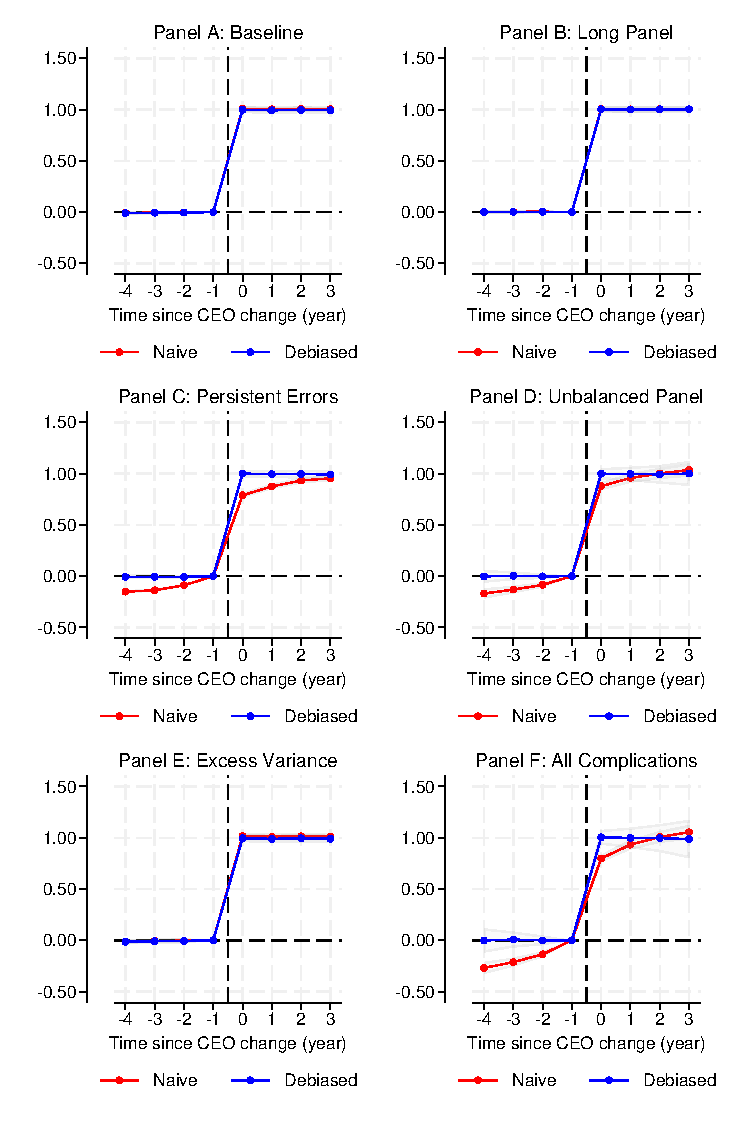
\includegraphics[width=0.95\textwidth]{figure/figuremc.pdf}
\caption{Monte Carlo event studies under six scenarios. Panels: Baseline, Long Panel, Persistent Errors, Unbalanced Panel, Excess Variance, All Complications. Bands are truncated to [-0.75, 1.75] for readability. [[comment: add precise definitions for beta0, beta1, dbeta from the estimator]]}
\label{fig:mc}
\end{figure}

\paragraph{Interpreting Table~\ref{tab:mc_params} and Figure~\ref{fig:mc}.}
Table~\ref{tab:mc_params} reports six Monte Carlo calibrations with different parameters. The baseline is very simple: balanced panels and i.i.d. (uncorrelated) error terms. Across scenarios we focus on four statistics that are widely used in applications: (i) the variance of the change in the manager fixed effect when the firm moves from the first to the second CEO, a key input to variance decompositions; (ii) the covariance of the revenue change at two years after the CEO change with the change in the manager fixed effect, which is the key component in regression slopes; (iii) an event-study slope two full years after the CEO change (the third post year), which captures dynamic adjustment; and (iv) a pre-trend coefficient two years before the change, which should be zero in the data-generating process once the baseline year $t=-1$ is normalized to zero. The debiasing is designed to remove finite-sample noise in all four statistics.

In the baseline, the naive variance is upward biased, while the debiased variance of the manager-effect change recovers exactly 1.00, which is the true value by construction. The covariance of the revenue change at year $+2$ with the change in the manager fixed effect is also upward biased in the naive estimate, but by exactly the same proportion as the variance. This proportional inflation occurs because when shocks are independent and identically distributed, the bias in both the numerator and denominator of the regression slope scales identically. As a consequence, the naive regression coefficient $\hat\beta_2$ is unbiased even though both its components are biased. This is a knife-edge case that holds only when $\rho$ is exactly zero. The debiased estimates recover the true covariance of 1.00 and the true slope of 1.00. Even in this favorable scenario, however, the $R^2$ remains upward biased because it is a nonlinear transformation of second moments. The long-panel scenario (spells of length 20) shows that all biases essentially disappear; this is a small-sample phenomenon in short panels.

With persistent errors ($\rho=0.9$), the naive variance is severely upward biased (about 100\% in our calibration), and spurious pre-trends emerge: before the manager arrives, the naive estimate suggests a negative effect. Because this is a Monte Carlo, we know the true pre-trend is zero; the bias is entirely mechanical. The covariance is also upward biased, but by a smaller factor (about 80\%) than the variance. This differential inflation breaks the proportionality that held under i.i.d. shocks: the bias now depends on the specific autocorrelation structure, not just the spell design. As a result, the naive post-arrival slope $\hat\beta_2$ at $+2$ is below one (about 0.90), consistent with a gradual, biased buildup. Debiasing removes the pre-trend, recovers the true covariance and variance, and delivers a post-arrival slope indistinguishable from the true value of 1.00.

The unbalanced-panel scenario (with a 20\% annual hazard of CEO change) compounds persistence and varying spell lengths. We again see a severe upward bias in the variance and evidence of pre-trends in the naive estimates. Debiasing removes these artifacts. Post-arrival dynamics look less gradual than under persistence alone, plausibly because typical spells are shorter in unbalanced panels, leaving less time for any gradual buildup to manifest.

In the excess-variance scenario, the treated group has higher shock variance than controls. Relative to the baseline, this produces more dispersion and a modest upward bias in the naive post-arrival slope; the debiased estimates correct both. Finally, the “all complications” scenario combines short and unbalanced spells, persistent errors, and excess variance. Here all problems are most severe: very large variance bias, pronounced pre-trends before the CEO arrives, and distorted dynamics. Yet the placebo correction handles them jointly: the debiased variance matches 1.00, the post-arrival slope is 1.00, and the pre-trend is 0.00 across all six scenarios. [[note: if you want exact standard errors or scenario-specific percent deviations tabulated, we can add them once the csv outputs are finalized.]]

Figure~\ref{fig:mc} displays event-study slopes for the same six scenarios. The motivation for plotting these is that, with persistent errors and/or unbalanced panels—both common in applications—noise can introduce apparent pre-trends. Researchers routinely check pre-trends, either formally or informally, and may be misled if naive profiles are biased.

Panel A (baseline) shows little bias: differences between naive and debiased lines are barely visible. Panel B (long panel) confirms that bias vanishes with long spells. Panel C (persistent errors) is the key case: the naive profile displays pre-trends and a somewhat sluggish post-arrival adjustment. The intuition is that the naive estimator uses estimated fixed effects that embed noise. With persistence, firms that happen to draw positive shocks over the post period are more likely to be classified as receiving a “good” CEO; by the same logic, their recent past is mechanically below average, generating a spurious pre-trend. The placebo correction strips out precisely this noise component.

Panels D–F illustrate that the problems intensify with unbalanced spells and excess variance, and are most severe when all complications are present. The true event study is the debiased (placebo-corrected) line: it jumps from 0 at $t=0^{-}$ to 1 at $t=0^{+}$ and stays flat thereafter. By contrast, the naive profiles can show strong pre-trends and distorted post dynamics. [[note: confirm which color/style corresponds to naive vs debiased in the final figure legend.]]

\section{Application: CEO Arrivals and Revenue in Hungarian Firms}

We apply the placebo-controlled debiasing to the universe of Hungarian firms, focusing on CEO arrivals and firm revenue outcomes. The Hungarian data provide an ideal setting because we observe the full population of businesses over three decades, not only large corporations. This scope yields many CEO mobilities across firms, allowing us to study the arrival of new CEOs and the associated within-firm dynamics. We document the data construction, sample restrictions, and additional statistics in our companion paper [[note: add citation to companion paper]]. Here we summarize the minimal features needed for this methodological application and outline the design we will estimate.

We consider all CEO changes between 1992 and 2022 (31 years). We restrict to firms that have ever reached at least 5 employees in their lifetime, to exclude non-employer businesses that rarely change CEOs and would inflate the sample numerically without adding identifying transitions. After this restriction, there are about 60,000 CEO changes [[note: update exact count]]. Many transitions are from the first to the second CEO and from founders to non-founders; these categories are similar but not identical because founders can return later and some firms begin with outsider CEOs. We will include a table with summary statistics for these quantities [[note: add exhibit reference]].

Identification relies on random mobility (strict exogeneity): past and future shocks to outcomes are orthogonal to CEO mobility timing. Because applied work commonly examines pre-trends to assess plausibility, we present event-study profiles grounded in this assumption.

We use firm revenue as the outcome variable for clarity of exposition. We remove industry–year means so that the outcome is measured as a deviation from the sectoral environment.

\subsection*{Estimating CEO Spell Effects}
For each transition from CEO A to CEO B, let the firm have two consecutive spells covering the entire tenures of A and B (not just the event window). We estimate a spell-level CEO effect as the within-spell mean of demeaned revenue. Concretely, let \(r_{it}\) denote firm revenue and let \(\tilde r_{it}=r_{it}-\bar r_{st}\) be revenue demeaned by industry–year \((s,t)\) cells. Let \(\mathbb 1\{\text{spell}=s\}\) indicate the A or B spell. The spell effect is
\begin{equation}
\hat z_{is} = \frac{1}{T_{is}}\sum_{t\in s} \tilde r_{it},\qquad s\in\{A,B\}.
\end{equation}
Define the change in the CEO effect for transition \(i\) by
\begin{equation}
\Delta \hat z_i = \hat z_{iB} - \hat z_{iA}.
\end{equation}
This statistic is the core object in variance decompositions; by theory and by Monte Carlo, its variance is upward biased in short panels and under persistence, which motivates our placebo debiasing.

[[note: if a firm has more than two consecutive spells, we treat adjacent spell pairs as separate transitions; multiple transitions per firm are allowed but clustered at the firm level.]]

\subsection*{Event-Study Specification}
We then study revenue dynamics around CEO arrivals in event time. For each transition with event date \(g\), define dummies for event-time leads/lags relative to \(g\) over the window \([-4,+3]\). We estimate
\begin{equation}
\tilde r_{it} = \alpha_i + \sum_{\ell\in\{-4,-3,-2,0,1,2,3\}} \beta_{\ell}\,\mathbb 1\{t-g=\ell\} + \varepsilon_{it},
\end{equation}
with the baseline period normalized to zero at \(t=-1\). The coefficients \(\beta_{\ell}\) trace out the revenue response before and after CEO arrival. Under random mobility, we expect no pre-trends: \(\beta_{-4},\beta_{-3},\beta_{-2}\approx 0\). Post-arrival dynamics are a question for the data: effects may be immediate or build gradually during the new CEO’s tenure. We will report both naive and placebo-corrected profiles; the latter subtract the corresponding placebo moments computed on matched non-changers with replicated spell designs.

\subsection*{Placebo Construction and Debiasing}
Placebo transitions assign a fake CEO change at the same calendar year as an actual transition to control firms that remain under the same CEO and have long no-change runs covering the event window. We split these control runs into the same pre/post spell lengths as the treated transition and align them in event time. Because the design matrices and weights are the same by construction, and because we assume the error autocovariance (\(\Sigma\)) is the same up to a scalar between treated and placebo groups, the covariance and variance bias components can be “precomputed” in the placebo sample and subtracted from the treated estimates. This delivers debiased variance of \(\Delta \hat z\) and debiased event-study coefficients \(\beta_{\ell}\).

[[note: add the companion paper citation for full data construction and additional outcomes (e.g., investment, materials, labor).]]

Hungary provides an ideal setting for studying CEO effects in the universe of private firms. The country offers complete administrative data coverage for all incorporated businesses, spanning 30 years from the transition economy of the 1990s through EU accession in 2004 to the present. CEO registration is mandatory for every registered firm. The coverage enables us to track CEO careers across firms and construct mobility networks necessary for identification.

Our analysis combines two administrative datasets. The firm registry, maintained by Hungarian corporate courts, contains records on all company representatives — individuals authorized to act on behalf of firms. These records include CEOs and other executives with signatory rights, tracked through a temporal database where each entry reflects representation status over specific time intervals. Updates occur when positions change, personal identifiers are modified, or reporting standards evolve. The registry provides names, addresses, dates of birth (from 2010), and mother's names (from 1999), though numerical identifiers exist only from 2013 onward.

The balance sheet dataset contains annual financial reports for all Hungarian firms with double-entry bookkeeping. The data has information on financial variables and some additional information, such as sector of activity, employment, and ownership (state, domestic, foreign). The two datasets cover 1,063,172 firms over 31 years, yielding 9,627,484 firm-year observations before sample restrictions.

Constructing CEO time series across firms poses some challenges. Before 2013, no numerical identifiers existed, requiring entity resolution based on names, addresses, mother's names, and birthdates. We link records across these dimensions to create unique person identifiers, enabling tracking across firms and over time. Matching quality improves after 1999 (when mother's names reporting begins) and 2010 (when birthdates reporting starts), though the 1990s data achieves reasonable coverage through name and address matching. 

Finding CEOs among all individuals from the data requires heuristics since job titles are inconsistently recorded. When explicit ``managing director'' titles exist, we use them directly. For remaining cases, we assume all representatives are CEOs if three or fewer exist at the firm. When more than three representatives are present, we assign CEO status based on continuity with previously identified CEOs. Time spans between appointments are often unclosed or non-contiguous, requiring imputation based on sequential information, assuming representatives remain active if their tenure includes June 21 of each year.

We apply several restrictions to create a sample suitable for productivity analysis. First, we exclude mining and finance sectors due to specialized accounting frameworks and regulatory environments. Second, we drop firms ever having more than 2 simultaneous CEOs to avoid complex governance structures that complicate identification. Third, we exclude firms with more than 10 CEO changes over the sample period (removing observations for unstable firms) to reduce noise from misclassified transitions. Fourth, we remove all state-owned enterprises, as their objectives and constraints differ from private businesses \citep{orban2019inception, shleifer1994politicians}.

We restrict attention to firms that employ at least 5 workers at some point in the firm lifecycle. This filter removes a substantial portion of observations but eliminates shell companies, tax optimization vehicles, and self-employment arrangements masquerading as corporations. The remaining firms represent genuine businesses with meaningful economic activity where management quality affects performance.

We exclude public firms and joint-stock companies from our analysis. The few companies traded on the Budapest Stock Exchange operate under different governance structures, compensation schemes, and disclosure requirements than private businesses. We also exclude cooperatives and other non-standard corporate forms where multiple managing directors share executive authority, as these organizational structures complicate identification of individual CEO effects.

Firms with multiple CEO changes are handled by splitting their history into adjacent transition pairs. After collapsing firm-CEO spells, intermediate spells are duplicated so that a firm with spells 1/2/3 contributes two transitions, 1$\to$2 and 2$\to$3. Each transition defines a pseudo-firm, indexed by a constructed identifier that groups the true firm with the relevant spell window. Fixed effects are estimated separately for these pseudo-firms, so outcomes around different transitions are allowed to have distinct firm intercepts. These pseudo-firms are not treated as independent statistical units. We retain the original firm identifier and cluster standard errors by the true firm. 

Appendix Table \ref{tab:sample} presents the number of firms in our sample relative to the total number of firms in the data for several year along the time series. The number of Hungarian firms increases abruptly during the nineties and also in the first 15 years of 2000s, albeit at a smaller pace.  The result of dropping the small firms results in using about one quarter of all firms. In the first year of study (1992) we have 26 thousand firms which increases to 115 thousand towards the end of the period. Overall, we have over one million firms and almost 10 million firm-years in the sample. The table also shows the number of CEOs each year, which presents a similar pattern; in 1992 we observe 32 thousand CEOs and in 2022 122 thousand. The total number of distinct CEOs is 340 thousand. Appendix Table \ref{tab:industry_stats} shows the industrial distribution of firms and CEOs. The largest sectors are Wholesale-Retail, Telecom and Business Services and Nontradable Services. 

Table \ref{tab:CEO_desc} shows the proportion of firms (and firm-years) by the number of CEOs observed in the firm during the period of observation. Not surprisingly, a majority of firms have only one CEO: 63\% of firms and 80\% of firm-years belong to this category. One quarter of firms had two CEOs while 13\% at least three CEOs. This latter category comprises only 3\% of firm-years. CEO spell lengths follow an exponential distribution with a 20 percent annual hazard rate, implying typical tenures of 3-7 years.


%%%%%%%%%%%%%%%%%
\section{Results}
%%%%%%%%%%%%%%%%% 

We present event studies examining revenue dynamics around CEO transitions. Figure \ref{fig:application} displays four key moments around CEO arrivals: variance of revenue changes (Panel A), the share of revenue variance explained by CEO transitions (Panel B), covariance of revenue with CEO effects (Panel C), and regression coefficients (Panel D). Each panel compares naive OLS estimates (red) with placebo-corrected debiased estimates (blue).

\begin{figure}[htbp]
\centering
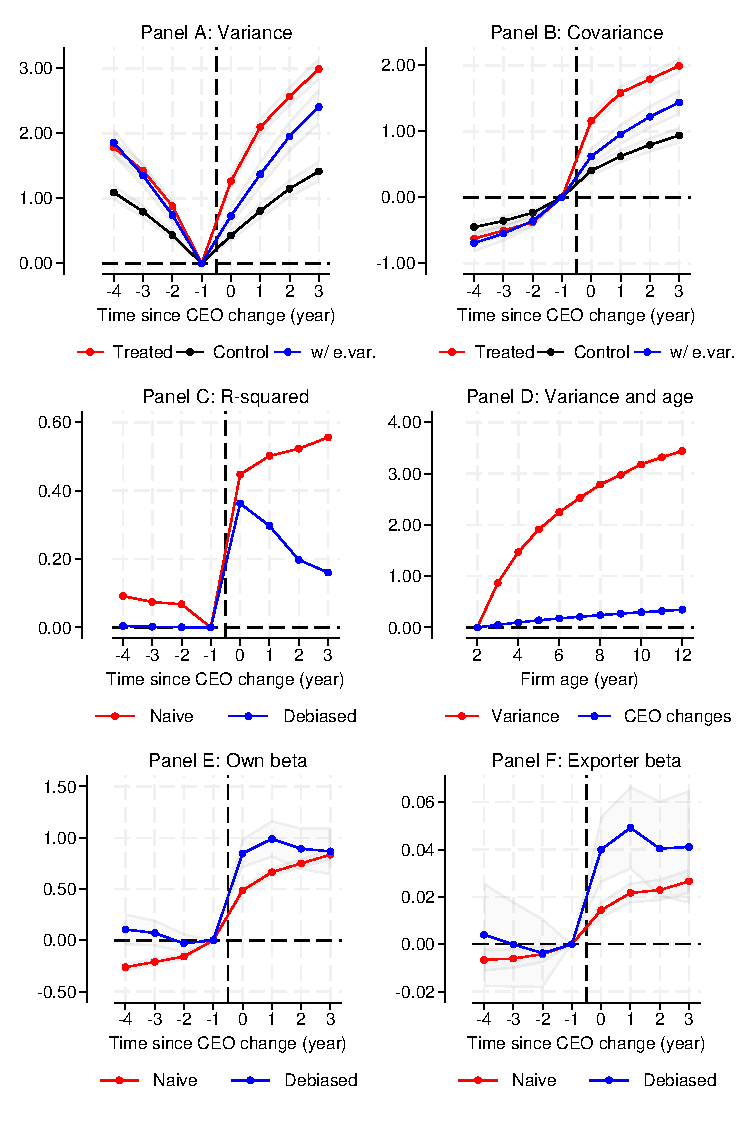
\includegraphics[width=0.95\textwidth]{figure/application.pdf}
\caption{Revenue Dynamics Around CEO Transitions in Hungarian Firms}
\label{fig:application}
\begin{minipage}{0.95\textwidth}
\footnotesize
Notes: Event studies of log revenue around CEO transitions. All panels normalize to year $t=-1$ (one year before CEO arrival). Panel A shows the variance of revenue changes from baseline. Panel B displays the fraction of revenue variance explained by CEO fixed effects (R-squared). Panel C plots the covariance of revenue change with the change in CEO fixed effect. Panel D shows regression coefficients from projecting revenue on CEO effects. Red lines show naive OLS estimates; blue lines show placebo-corrected debiased estimates. Shaded regions indicate 95\% confidence intervals. The placebo group consists of matched non-changing firms from the same birth cohort and sector, assigned pseudo CEO transitions at the same calendar year as treated firms. Event window spans $[-4, +3]$ years around CEO arrival.
\end{minipage}
\end{figure}

\paragraph{Variance of Revenue Changes (Panel A).} Panel A displays the variance of the change in log revenue by event time. The naive estimate (red) is severely upward biased, particularly in the post-transition period. There is also a pretrend, which is natural: at times farther away from the baseline year $t=-1$, the variance of revenue changes mechanically increases due to accumulating shocks.The debiased estimate (blue) removes this mechanical noise. The debiased variance remains constant before the CEO arrival, and jumps to about 1 after arrival. There is a partial adjustment in the first year, but this is expected since some CEOs arrive mid-year. 

\paragraph{Covariance of Revenue with CEO Effects (Panel B).} Panel B shows the covariance of the revenue change with the change in CEO fixed effects, a key component in event-study regressions. The naive estimate (red) displays strong spurious pre-trends: before the CEO arrives, past revenue changes appear correlated with future CEO quality. The debiased estimate (blue) shows that the pretrend is entirely spurious and there is no significant pretrend. After the CEO arrives, covariance becomes positive and stable. Again, the first year shows partial adjustment, but covariance stabilizes thereafter. 

\paragraph{Variance Decomposition (Panel C).} Panel C translates the variance and covariance estimates into an $R^2$: the fraction of revenue variance explained by CEO fixed effects. This statistic should be zero before the CEO arrives, since future CEO identity cannot explain past outcomes. The debiased estimate confirms this. After the CEO arrives, the naive estimate suggests CEO effects explain 40--60\% of revenue variance. The debiased estimate shows an $R^2$ of 20--30\%---substantial, but only half the naive estimate. This decomposition demonstrates that ignoring small-sample bias dramatically overstates the role of CEOs in firm performance.

\paragraph{Variance Decomposition by Firm Age (Panel D).} Using the estimated variance of CEO fixed effects, we can compute how much CEOs contribute to revenue variance by firm age. Assuming that each CEO change adds the same variance to log revenue, we can back out the variance of CEO effects by age group. As firms age, they accumulate revenue shocks (red), but they also tend to change CEOs more often (blue). Over time, about a tenth of revenue variance is explained by CEO effects. This is smaller than the $R^2$ reported in Panel C because older firms have more accumulated shocks, diluting the relative contribution of CEOs.

\paragraph{Regression Coefficients (Panel E).} Panel E rescales the covariance and the variance of the CEO fixed effect into regression slopes, measuring the elasticity of revenue with respect to CEO quality. This is a nonlinear transformation, so we compute standard errors via the delta method. The naive estimate shows pronounced pre-trends and a gradual post-arrival buildup. The debiased estimate eliminates the pre-trend and reveals almost immediate, persistent effects. 

\paragraph{Regression of Exporter Status on CEO Quality (Panel F).} Panel F extends the analysis to a binary outcome: whether the firm exports. We estimate a linear probability model of exporter status on CEO fixed effects in event time. The naive estimate shows slow adjustment after CEO arrival, while the debiased estimate reveals an immediate jump in export probability. CEOs appear to have a substantial impact on firms' international engagement, with a 10\% better CEO increasing export likelihood by 0.4--0.6 percentage points.


%%%%%%%%%%%%%%%%%%%%
\section{Conclusion}
%%%%%%%%%%%%%%%%%%%%

This paper estimates the contribution of CEOs to firm revenue by exploiting a unique administrative dataset covering the entire population of Hungarian private firms and their CEOs from 1992 to 2022. The novelty of the data lies in its unprecedented scope and completeness, allowing the study of CEO effects not only in large firms but crucially in small and medium-sized enterprises that dominate every economy. The combination of the dataset with a theoretically grounded placebo-controlled method allows for a more precise attribution of CEO effects. 

The paper develops a new placebo-controlled event study design that overcomes limited mobility bias, which contaminates studies using two fixed effects.  By creating matched placebo CEO transitions in firms without actual leadership changes, the method effectively separates true CEO skill effects on revenue from mechanical noise. Empirically, the findings reveal that the true causal effect of CEO quality on firm revenue is economically meaningful but notably smaller than raw correlations suggest, explaining about 29 percent of revenue variation after correction. 

An alternative way to deal with the noise problem is to use observable manager characteristics as measures of skill. Observable characteristics such as education and work experience \citep{DePirro2025}, foreign name as a proxy for international exposure \citep{Koren2023expat}, and the selectiveness of entry cohorts \citep{koren2024managers} offer more reliable, though narrower, measures of specific dimensions of managerial quality. These observables capture only partial aspects of CEO ability but avoid the mechanical noise that contaminates fixed effects estimates.

\clearpage
\bibliographystyle{apalike}
\bibliography{lib/references}

\clearpage
\appendix
\renewcommand{\thefigure}{A\arabic{figure}}
\renewcommand{\thetable}{A\arabic{table}}
\setcounter{figure}{0}
\setcounter{table}{0}

\section{Derivation of Bias Terms}

This appendix provides the formal matrix algebra derivation of the bias terms in second moments of estimated CEO effects.

\subsection{Matrix Notation Setup}

\paragraph{Model setup.} Let firm $i$ be observed for $T$ periods with outcome path $\mathbf y_i\in\mathbb R^T$ that decomposes into a (piecewise-constant) manager-effect path $\mathbf z_i$ and shocks $\mathbf e_i$. Suppose manager 1 serves in the first $T_1$ periods and manager 2 in the last $T_2=T-T_1$ periods. (Other transition paths can be modeled similarly.) The model is
\begin{equation}
\mathbf y_i = \mathbf z_i + \mathbf e_i
\end{equation}
with 
\begin{equation}
\mathbb E[\mathbf z_i\mathbf z_i']= \mathbf \Lambda_i=
\begin{bmatrix}
  \lambda_{i11}\otimes \mathbf{11}' & \lambda_{i12}\otimes \mathbf{11}'\\
  \lambda_{i12}\otimes \mathbf{11}' & \lambda_{i22}\otimes \mathbf{11}'
\end{bmatrix},
\qquad \mathbb E[\mathbf z_i\mathbf e_i']=0,
\qquad \mathbb E[\mathbf e_i\mathbf e_i']=\sigma_1\mathbf\Sigma
\end{equation}
for changing firms, and 
\begin{equation}
\mathbb E[\mathbf z_i\mathbf z_i']= \mathbf \Lambda_i=
  \lambda_{i11}\otimes \mathbf{11}',
\qquad \mathbb E[\mathbf z_i\mathbf e_i']=0,
\qquad \mathbb E[\mathbf e_i\mathbf e_i']=\sigma_0\mathbf\Sigma
\end{equation}
for non-changing firms. The first equation is notation for the variance and covariance of manager fixed effects at firm $i$. The second equation states strict exogeneity (random mobility): every period's shock is mean independent of the entire CEO path. The third assumption allows for arbitrary autocorrelation in shocks over time but assumes that this autocorrelation is the same for changing and non-changing firms, up to a scalar multiplier $\sigma_1/\sigma_0$ (proportional autocovariance).

\paragraph{Projection Matrix and LSDV Estimator.} Introduce a design matrix $\mathbf D$ to map rows to CEO spells. For the example with $T_1=2$ pre-spell periods and $T_2=3$ post-spell periods:
\[
  \mathbf D = \begin{bmatrix}
    1 & 0\\
    1 & 0\\
    0 & 1\\
    0 & 1\\
    0 & 1
  \end{bmatrix},
\]
and the diagonal matrix of spell lengths $\mathbf T$ as
$$
  \mathbf T = \operatorname{diag}(T_1,T_2)=\operatorname{diag}(2,3).
$$
The projection matrix that converts outcomes to within-spell means is
$$
  \mathbf P = \mathbf D\,\mathbf T^{-1}\,\mathbf D'.
$$
In the example,
\[
  \mathbf P = \begin{bmatrix}
    1/2 & 1/2 & 0 & 0 & 0\\
    1/2 & 1/2 & 0 & 0 & 0\\
    0 & 0 & 1/3 & 1/3 & 1/3\\
    0 & 0 & 1/3 & 1/3 & 1/3\\
    0 & 0 & 1/3 & 1/3 & 1/3
  \end{bmatrix}\quad\Rightarrow\quad
  \mathbf {Py}_i = 
  \begin{pmatrix}
  \frac12 \sum_{t=-2}^{-1} y_{it} \\
  \frac12 \sum_{t=-2}^{-1} y_{it} \\
  \frac13 \sum_{t=0}^{+2} y_{it}\\
  \frac13 \sum_{t=0}^{+2} y_{it}\\
  \frac13 \sum_{t=0}^{+2} y_{it}
  \end{pmatrix}.
\]
Note that $\mathbf P$ is idempotent ($\mathbf P^2=\mathbf P$) and symmetric ($\mathbf P'=\mathbf P$). We also have $\mathbf P\mathbf z_i = \mathbf z_i$ because $\mathbf z_i$ is piecewise constant within spells.

The least-squares dummy variable (LSDV) estimator of the CEO effects is
\begin{equation}\label{eq:lsdv_appendix}
  \hat{\mathbf z}_i = \mathbf P\mathbf y_i = \mathbf z_i + \mathbf P\mathbf e_i.
\end{equation}  
The estimated CEO effects are the true effects plus the within-spell mean of shocks.

\subsection{Population Moments and Bias Terms}

The estimator is unbiased but is only consistent as spell lengths grow large. The small-sample noise contaminates all second moments of $\hat{\mathbf z}_i$. The relevant moments are
\begin{align}
  \mathbb E[\hat{\mathbf z_i}] &= \mathbf z_i,\\
  \mathbb E[\hat{\mathbf z_i}\hat{\mathbf z_i}'] &= 
\mathbb E[(\mathbf z_i + \mathbf P\mathbf e_i)(\mathbf z_i + \mathbf P\mathbf e_i)' ] =
    \mathbf \Lambda_i + \sigma\mathbf P\mathbf\Sigma\mathbf P,\\ 
  \mathbb E[\hat{\mathbf z_i}\mathbf e_i'] &= 
\mathbb E[(\mathbf z_i + \mathbf P\mathbf e_i)\mathbf e_i' ] = \sigma\mathbf P\mathbf\Sigma,\\
  \mathbb E[\hat{\mathbf z_i}\mathbf y_i'] &= 
\mathbb E[(\mathbf z_i + \mathbf P\mathbf e_i)(\mathbf z_i + \mathbf e_i)' ] = \mathbf \Lambda_i + \sigma\mathbf P\mathbf\Sigma.
\end{align}
The first equation restates unbiasedness. The second equation shows that the variance-covariance of estimated CEO effects is inflated by the term $\sigma\mathbf P\mathbf\Sigma\mathbf P$ relative to the true variance-covariance $\mathbf \Lambda_i$. The third equation shows that the covariance of estimated CEO effects with shocks is contaminated. The fourth equation shows that the covariance of outcomes with estimated CEO effects is also inflated.

\subsection{Bias in Regression Slopes}

For any linear contrast with weights $\mathbf w\in\mathbb R^T$ and $\mathbf w'\mathbf 1=0$, define the estimated effect for the contrast by
$$
\Delta\hat z_i = \mathbf w'\hat{\mathbf z}_i = \mathbf w'\mathbf P\,\mathbf y_i = \Delta z_i + \eta_i,\qquad \eta_i:=\mathbf w'\mathbf P\,\mathbf e_i,
$$
and recall that $\Delta y_i = \Delta z_i + \varepsilon_i$ where $\varepsilon_i=\mathbf w'\mathbf e_i$. 

The naive regression slope is
\begin{equation}
\hat\beta = 
  \frac {\Cov(\Delta \hat z_i, \Delta y_i)}
        {\Var(\Delta \hat z_i)} =
  \frac {\mathbf w' \mathbb E[\hat{\mathbf z_i}\mathbf y_i ']\mathbf w}
        {\mathbf w' \mathbb E[\hat{\mathbf z_i}\hat{\mathbf z_i}']\mathbf w} =
  \frac {\mathbf w' [\mathbf \Lambda_i + \sigma \mathbf P\mathbf\Sigma]\mathbf w}
        {\mathbf w' [\mathbf \Lambda_i + \sigma \mathbf P\mathbf\Sigma\mathbf P]\mathbf w} =
  \frac {\lambda_i + \sigma \mathbf w' \mathbf P\mathbf\Sigma \mathbf w}
        {\lambda_i + \sigma \mathbf w' \mathbf P\mathbf\Sigma \mathbf P \mathbf w}. 
\end{equation}  

\textit{Covariance bias term.} $\Cov(\varepsilon_i,\eta_i)$ is typically positive because both $\varepsilon_i$ and $\eta_i$ are formed from the same underlying shocks averaged over overlapping windows (short spells and persistent shocks make this more pronounced). This inflates the numerator.

\textit{Variance bias term (classical measurement error).} $\Var(\eta_i)>0$ inflates the denominator, the standard attenuation channel.

Together, the slope can be biased up or down depending on the balance between these terms. With i.i.d. shocks and long, balanced spells, $\Cov(\varepsilon_i,\eta_i)\approx 0$ and $\Var(\eta_i)$ is small. Both components are small-sample phenomena driven by short $T_1$ and $T_2$. As $T_1,T_2\to\infty$, spell means average out shocks so both bias terms vanish.

\subsection{Sample Moments Across Heterogeneous Groups}

In practice, we estimate the population moments using sample analogs. There are $G$ groups with different spell lengths and contrasts (e.g., different event windows). Within each group $g$, we observe $N_g$ firms with outcomes $\{\Delta y_i, \Delta \hat z_i\}_{i=1}^{N_g}$. The sample moments are
\begin{align}
\widehat{\Cov}(\Delta y_i,\Delta \hat z_i) &= \sum_{g=1}^G \frac{N_g}{N} \widehat{\Cov}_g(\Delta y_i,\Delta \hat z_i)\\
\widehat{\Var}(\Delta \hat z_i) &= \sum_{g=1}^G \frac{N_g}{N} \widehat{\Var}_g(\Delta \hat z_i)
\end{align}

The expected values are
\begin{align}
\mathbb E\widehat{\Cov}(\Delta y_i,\Delta \hat z_i) &= \sum_{g=1}^G \frac{N_g}{N} \left[ 
\Bar\lambda_g
+ \sigma_g \mathbf w_g' \mathbf P_g\mathbf\Sigma \mathbf w_g\right] = 
\Bar\lambda +\sum_{g=1}^G \frac{N_g}{N} \sigma_g \mathbf w_g' \mathbf P_g\mathbf\Sigma \mathbf w_g\\
\mathbb E\widehat{\Var}(\Delta \hat z_i) &= \sum_{g=1}^G \frac{N_g}{N} \left[ 
\Bar\lambda_g
+ \sigma_g \mathbf w_g' \mathbf P_g\mathbf\Sigma \mathbf P_g \mathbf w_g\right] = 
\Bar\lambda +\sum_{g=1}^G \frac{N_g}{N} \sigma_g \mathbf w_g' \mathbf P_g\mathbf\Sigma \mathbf P_g \mathbf w_g
\end{align}

Here $\Bar\lambda_g$ is the average variance of CEO effects in group $g$, and $\Bar\lambda$ is the overall average variance of CEO effects across all groups. Without the bias, the sample covariance and variance would identify the average treatment effect $\Bar\lambda$ even with heterogeneous groups.

The bias terms are complicated group averages that depend on the design matrices $\mathbf P_g$, the weight vectors $\mathbf w_g$, and the shock structure $\sigma_g\mathbf\Sigma$. It is often impractical to estimate these components directly, especially when $\mathbf\Sigma$ is complex (e.g., persistent shocks) and when there are many groups with different designs.

\section{Additional Tables and Figures}

%Benne maradhat a populáció, de kellene a minta is. Esetleg kidobhatjuk a firms oszlopot, és készítsük el a táblát a populációra és a mi mintánkra (Population: firm-year CEO, Sample: firm-year CEO, Surplus Share)


%\begin{table}[htbp]\centering
\def\sym#1{\ifmmode^{#1}\else\(^{#1}\)\fi}
\caption{Surplus Function Estimation Results}
\begin{tabular}{l*{6}{c}}
\toprule
                    &\multicolumn{1}{c}{(1)}&\multicolumn{1}{c}{(2)}&\multicolumn{1}{c}{(3)}&\multicolumn{1}{c}{(4)}&\multicolumn{1}{c}{(5)}&\multicolumn{1}{c}{(6)}\\
                    &\multicolumn{1}{c}{Revenue}&\multicolumn{1}{c}{EBITDA}&\multicolumn{1}{c}{Wagebill}&\multicolumn{1}{c}{Materials}&\multicolumn{1}{c}{Revenue}&\multicolumn{1}{c}{Revenue}\\
\midrule
Fixed assets (log)  &       0.323\sym{***}&       0.325\sym{***}&       0.287\sym{***}&       0.375\sym{***}&       0.290\sym{***}&       0.295\sym{***}\\
                    &     (0.001)         &     (0.001)         &     (0.001)         &     (0.002)         &     (0.001)         &     (0.004)         \\
\addlinespace
Has intangible assets&       0.268\sym{***}&       0.163\sym{***}&       0.267\sym{***}&       0.317\sym{***}&       0.205\sym{***}&       0.255\sym{***}\\
                    &     (0.003)         &     (0.003)         &     (0.003)         &     (0.004)         &     (0.003)         &     (0.010)         \\
\addlinespace
Founding owner      &      -0.079\sym{***}&      -0.051\sym{***}&      -0.017\sym{***}&      -0.099\sym{***}&      -0.010\sym{***}&      -0.015\sym{*}  \\
                    &     (0.005)         &     (0.005)         &     (0.005)         &     (0.006)         &     (0.003)         &     (0.008)         \\
\addlinespace
Non-founding owner  &      -0.001         &      -0.000         &      -0.003         &      -0.006         &      -0.011\sym{***}&      -0.017\sym{*}  \\
                    &     (0.007)         &     (0.006)         &     (0.007)         &     (0.009)         &     (0.004)         &     (0.009)         \\
\addlinespace
Foreign owned       &       0.025\sym{**} &       0.018         &       0.064\sym{***}&       0.010         &       0.022\sym{*}  &       0.033         \\
                    &     (0.012)         &     (0.012)         &     (0.012)         &     (0.015)         &     (0.011)         &     (0.025)         \\
\addlinespace
State owned         &       0.148\sym{***}&       0.047\sym{*}  &       0.448\sym{***}&       0.146\sym{***}&       0.062\sym{**} &       0.050         \\
                    &     (0.029)         &     (0.028)         &     (0.029)         &     (0.032)         &     (0.026)         &     (0.059)         \\
\midrule
Observations        &     3004184         &     2326192         &     2949024         &     3059662         &     2967233         &      374084         \\
\bottomrule
\multicolumn{7}{l}{\footnotesize Standard errors in parentheses}\\
\multicolumn{7}{l}{\footnotesize All models include firm fixed effects, industry-year fixed effects, and a step function for firm age.}\\
\multicolumn{7}{l}{\footnotesize Outcome variables are log-transformed. Models (5) and (6) include quadratic controls for CEO age and tenure.}\\
\multicolumn{7}{l}{\footnotesize Model (6) restricts to largest connected component of CEO-firm network.}\\
\multicolumn{7}{l}{\footnotesize \sym{*} \(p<0.10\), \sym{**} \(p<0.05\), \sym{***} \(p<0.01\)}\\
\end{tabular}
\end{table}




\end{document}
